%--Copyright oldal----------------------------------------
\iffalse

\newpage\null\thispagestyle{empty}
\newpage\thispagestyle{empty}
Szerzői jog \textcopyright ~Knyihár Gábor, 2018.\\[2cm]

\begin{center}
    \bf ZÁRADÉK
\end{center}


{\bf Ez a szakdolgozat elzártan kezelendő és őrzendő, a hozzáférése a vonatkozó szabályok szerint korlátozott, a dolgozat tartalmát csak az arra feljogosí-tott személyek ismerhetik.}

{\bf A korlátozott hozzáférés időtartamának lejártáig az arra feljogosítottakon kívül csak a korlátozást kérelmező személy vagy gazdálkodó szervezet írásos engedélyéjével rendelkező személy nyerhet betekintést a dolgozat tartalmába.}\\[0.5cm]

{\bf A hozzáférés korlátozása és a zárt kezelés 2023. év december hónap 
31. napján ér véget.}

\fi

%--Feladatkiírás lapja------------------------------------
\newpage\null\thispagestyle{empty}
\centerline{Ide kell befűzni az eredeti feladatkiírási lapot!}
%\newpage\thispagestyle{empty}

%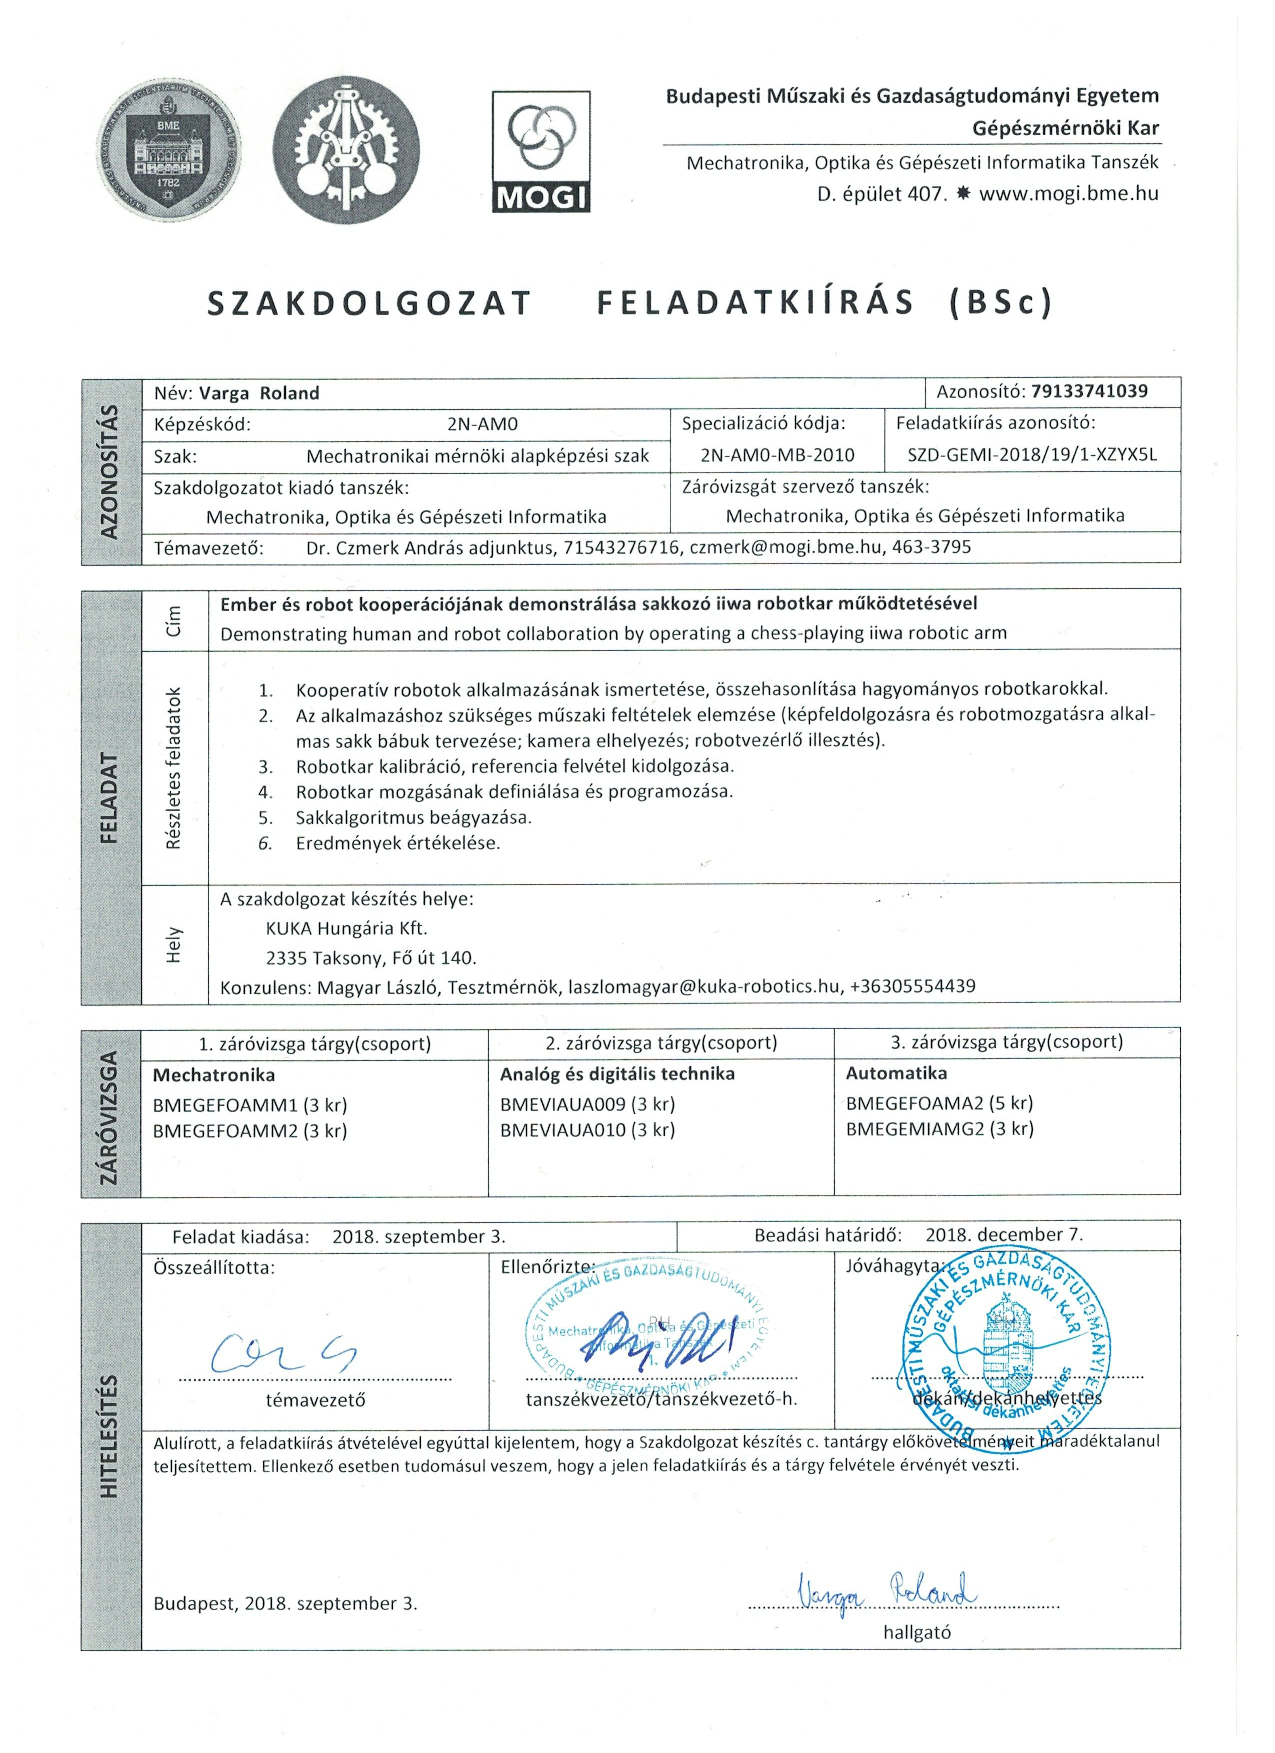
\includepdf[pages=-, offset=75 -75]{Figures/feladatkiiras.pdf}

%--Nyilatkozatok------------------------------------------
%\newpage\null\thispagestyle{empty}
\newpage\thispagestyle{plain}
\begin{center}
    \Large \MakeUppercase{Nyilatkozatok}
\end{center}

{\centering \itshape Beadhatósági nyilatkozat \par}
A jelen szakdolgozat az üzem által elvárt szakmai színvonalnak mind tartalmilag, mind formailag megfelel, beadható.

Kelt, 

{\hspace{0.4\textwidth} Az üzem részéről:}\\[1cm]

{\hspace{0.6\textwidth} \itshape üzemi konzulens}\\[0.1cm]

{\centering \itshape Elfogadási nyilatkozat \par}
Ezen szakdolgozat a Budapesti Műszaki és Gazdaságtudományi Egyetem Gépészmérnöki Kara által a Diplomatervezési és Szakdolgozat feladatokra előírt valamennyi tartalmi és formai követelménynek, továbbá a feladatkiírásban előírtaknak maradéktalanul eleget tesz. E szakdolgozatot a nyilvános bírálatra és nyilvános előadásra alkalmasnak tartom. 

A beadás időpontja: \\[1cm]

{\hspace{0.62\textwidth} \itshape témavezető}\\[0.1cm]

{\centering \itshape Nyilatkozat önálló munkáról \par}
Alulírott, Varga Roland (XZYX5L), a Budapesti Műszaki és Gazdaságtudományi Egyetem hallgatója, büntetőjogi és fegyelmi felelősségem tudatában kijelentem és sajátkezű aláírásommal igazolom, hogy ezt a szakdolgozatot meg nem engedett segítség nélkül, saját magam készítettem, és dolgozatomban csak a megadott forrásokat használtam fel. Minden olyan részt, melyet szó szerint vagy azonos értelemben, de átfogalmazva más forrásból átvettem, egyértelműen, a hatályos előírásoknak megfelelően, a forrás megadásával megjelöltem.

{Budapest, 2018 ......................}\\[1cm]

{\hspace{0.6\textwidth} \itshape szigorló hallgató}